\subsection{Results}

\begin{figure}
  %\centering
  %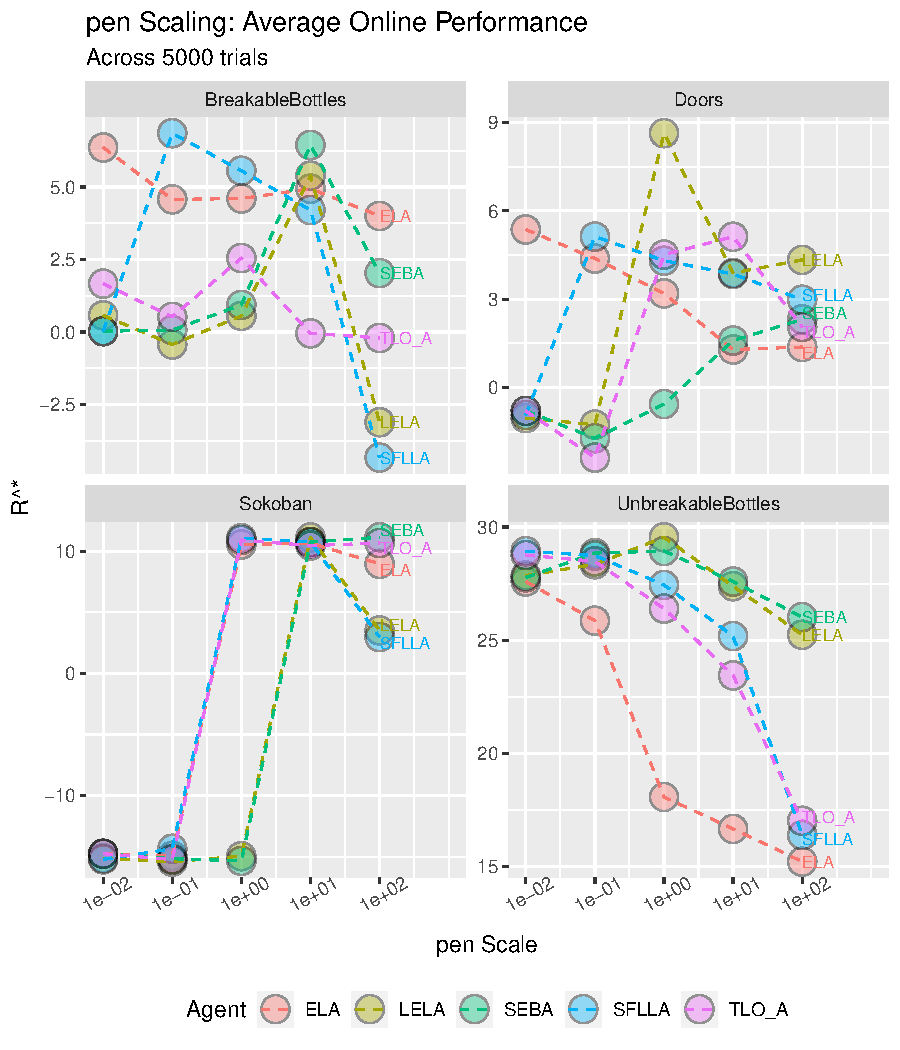
\includegraphics[width=\columnwidth]{output/onlinepen.pdf}
  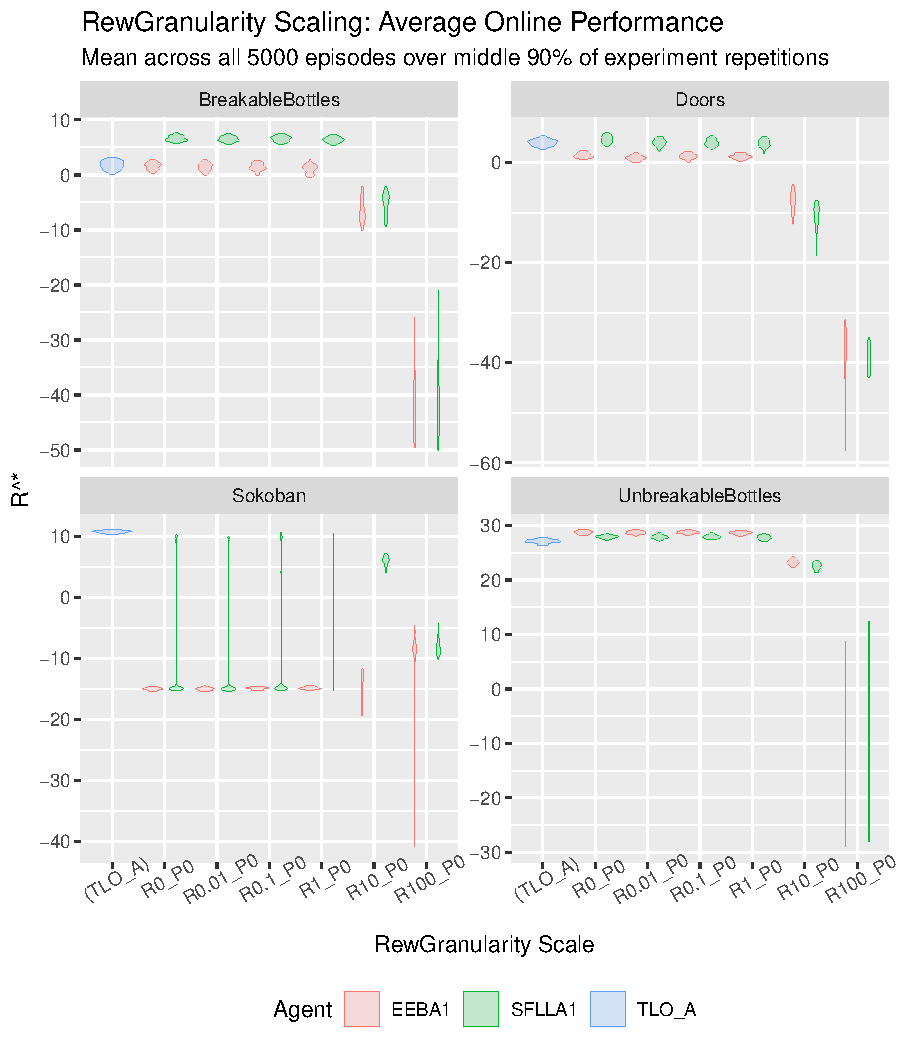
\includegraphics[width=\columnwidth]{output/multirun_n100_pilot_granularityonline_RewGranularity.pdf}
  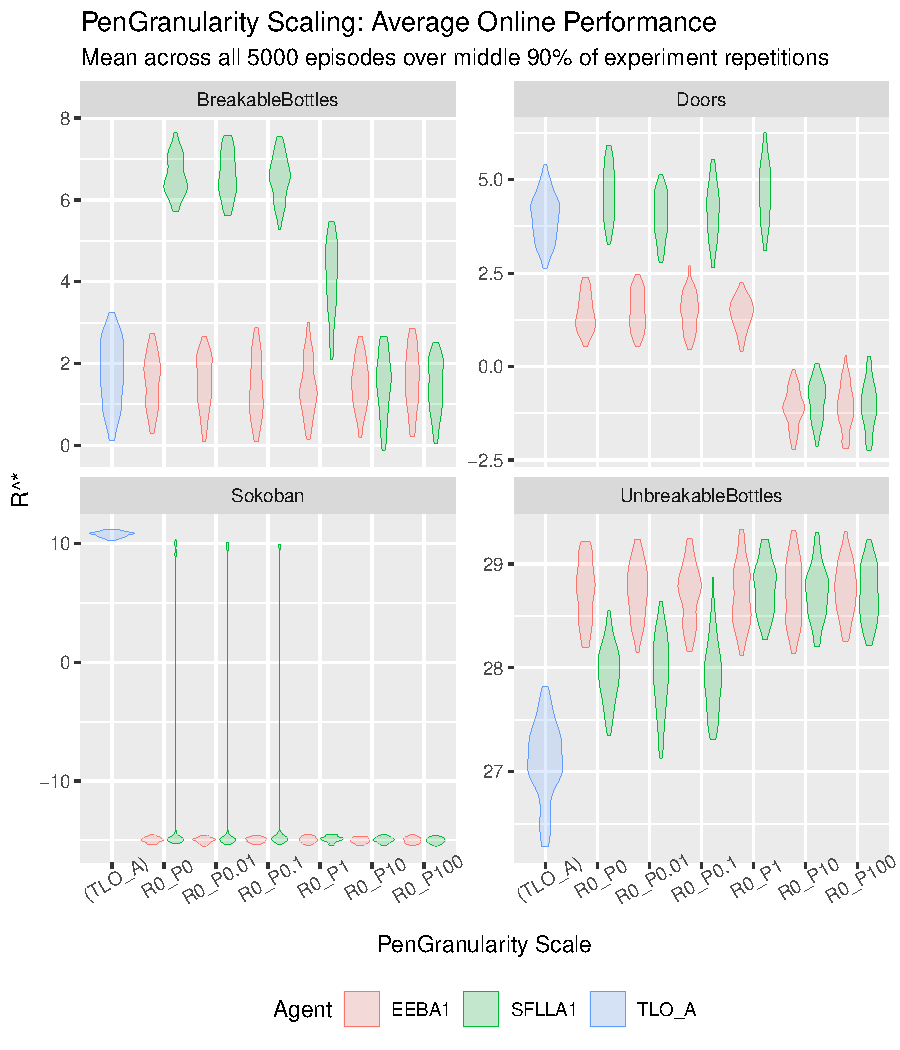
\includegraphics[width=\columnwidth]{output/multirun_n100_pilot_granularityonline_PenGranularity.pdf}
  \caption{By creating `granularity' for our non-linear transform agents, we can simulate similarity with $TLO_A$, which might be considered as a custom-tuned form of granularity.
  }
   \label{fig:exp3_main}
   \Description{By creating `granularity' for our non-linear transform agents, we can simulate similarity with $TLO_A$, which might be considered as a custom-tuned form of granularity.}
 \end{figure}
 
For SFELLA, as expected, performance declined as granularity increased, particularly in the BreakableBottles environment where it previously had a clear advantage over $TLO_A$ (Figure~\ref{fig:exp3_main}). For UnbreakableBottles, performance declined as granularity for the Reward Scaling was increased. In the Doors environment, performance declined, from signifantly better (???) than $TLO_A$ to much, much worse. In the Sokoban evnrionment, as in Expermetn 1, $TLO_A$ was the better performer and remained so.

The result confirms that where SFELLA performs well, it does so because it avoids `granularity' and is sensitive to changes in reward right across teh scale. In contrast, $TLO_A$ is sometimes insensitive to changes that exceed its threshold. Where it is well tuned, it performs well, or even better, than othere algorithms, but when not well-tunred, it performs less well.



